\documentclass[twoside]{book}

% Packages required by doxygen
\usepackage{fixltx2e}
\usepackage{calc}
\usepackage{doxygen}
\usepackage[export]{adjustbox} % also loads graphicx
\usepackage{graphicx}
\usepackage[utf8]{inputenc}
\usepackage{makeidx}
\usepackage{multicol}
\usepackage{multirow}
\PassOptionsToPackage{warn}{textcomp}
\usepackage{textcomp}
\usepackage[nointegrals]{wasysym}
\usepackage[table]{xcolor}

% Font selection
\usepackage[T1]{fontenc}
\usepackage[scaled=.90]{helvet}
\usepackage{courier}
\usepackage{amssymb}
\usepackage{sectsty}
\renewcommand{\familydefault}{\sfdefault}
\allsectionsfont{%
  \fontseries{bc}\selectfont%
  \color{darkgray}%
}
\renewcommand{\DoxyLabelFont}{%
  \fontseries{bc}\selectfont%
  \color{darkgray}%
}
\newcommand{\+}{\discretionary{\mbox{\scriptsize$\hookleftarrow$}}{}{}}

% Page & text layout
\usepackage{geometry}
\geometry{%
  a4paper,%
  top=2.5cm,%
  bottom=2.5cm,%
  left=2.5cm,%
  right=2.5cm%
}
\tolerance=750
\hfuzz=15pt
\hbadness=750
\setlength{\emergencystretch}{15pt}
\setlength{\parindent}{0cm}
\setlength{\parskip}{3ex plus 2ex minus 2ex}
\makeatletter
\renewcommand{\paragraph}{%
  \@startsection{paragraph}{4}{0ex}{-1.0ex}{1.0ex}{%
    \normalfont\normalsize\bfseries\SS@parafont%
  }%
}
\renewcommand{\subparagraph}{%
  \@startsection{subparagraph}{5}{0ex}{-1.0ex}{1.0ex}{%
    \normalfont\normalsize\bfseries\SS@subparafont%
  }%
}
\makeatother

% Headers & footers
\usepackage{fancyhdr}
\pagestyle{fancyplain}
\fancyhead[LE]{\fancyplain{}{\bfseries\thepage}}
\fancyhead[CE]{\fancyplain{}{}}
\fancyhead[RE]{\fancyplain{}{\bfseries\leftmark}}
\fancyhead[LO]{\fancyplain{}{\bfseries\rightmark}}
\fancyhead[CO]{\fancyplain{}{}}
\fancyhead[RO]{\fancyplain{}{\bfseries\thepage}}
\fancyfoot[LE]{\fancyplain{}{}}
\fancyfoot[CE]{\fancyplain{}{}}
\fancyfoot[RE]{\fancyplain{}{\bfseries\scriptsize Generated by Doxygen }}
\fancyfoot[LO]{\fancyplain{}{\bfseries\scriptsize Generated by Doxygen }}
\fancyfoot[CO]{\fancyplain{}{}}
\fancyfoot[RO]{\fancyplain{}{}}
\renewcommand{\footrulewidth}{0.4pt}
\renewcommand{\chaptermark}[1]{%
  \markboth{#1}{}%
}
\renewcommand{\sectionmark}[1]{%
  \markright{\thesection\ #1}%
}

% Indices & bibliography
\usepackage{natbib}
\usepackage[titles]{tocloft}
\setcounter{tocdepth}{3}
\setcounter{secnumdepth}{5}
\makeindex

% Hyperlinks (required, but should be loaded last)
\usepackage{ifpdf}
\ifpdf
  \usepackage[pdftex,pagebackref=true]{hyperref}
\else
  \usepackage[ps2pdf,pagebackref=true]{hyperref}
\fi
\hypersetup{%
  colorlinks=true,%
  linkcolor=blue,%
  citecolor=blue,%
  unicode%
}

% Custom commands
\newcommand{\clearemptydoublepage}{%
  \newpage{\pagestyle{empty}\cleardoublepage}%
}

\usepackage{caption}
\captionsetup{labelsep=space,justification=centering,font={bf},singlelinecheck=off,skip=4pt,position=top}

%===== C O N T E N T S =====

\begin{document}

% Titlepage & ToC
\hypersetup{pageanchor=false,
             bookmarksnumbered=true,
             pdfencoding=unicode
            }
\pagenumbering{roman}
\begin{titlepage}
\vspace*{7cm}
\begin{center}%
{\Large My Project }\\
\vspace*{1cm}
{\large Generated by Doxygen 1.8.11}\\
\end{center}
\end{titlepage}
\clearemptydoublepage
\tableofcontents
\clearemptydoublepage
\pagenumbering{arabic}
\hypersetup{pageanchor=true}

%--- Begin generated contents ---
\chapter{Class Index}
\section{Class List}
Here are the classes, structs, unions and interfaces with brief descriptions\+:\begin{DoxyCompactList}
\item\contentsline{section}{\hyperlink{structnode}{node} }{\pageref{structnode}}{}
\item\contentsline{section}{\hyperlink{structnode1}{node1} }{\pageref{structnode1}}{}
\item\contentsline{section}{\hyperlink{structnode__info}{node\+\_\+info} }{\pageref{structnode__info}}{}
\end{DoxyCompactList}

\chapter{File Index}
\section{File List}
Here is a list of all files with brief descriptions\+:\begin{DoxyCompactList}
\item\contentsline{section}{\hyperlink{Lab1_8c}{Lab1.\+c} }{\pageref{Lab1_8c}}{}
\end{DoxyCompactList}

\chapter{Class Documentation}
\hypertarget{classEquation}{}\section{Equation Class Reference}
\label{classEquation}\index{Equation@{Equation}}


{\ttfamily \#include $<$Equation.\+h$>$}



Collaboration diagram for Equation\+:
\nopagebreak
\begin{figure}[H]
\begin{center}
\leavevmode
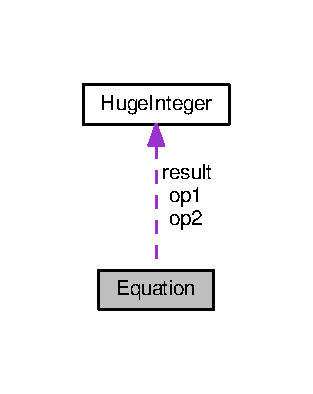
\includegraphics[width=150pt]{classEquation__coll__graph}
\end{center}
\end{figure}
\subsection*{Public Member Functions}
\begin{DoxyCompactItemize}
\item 
\hyperlink{classEquation_a68511fc719250ed80f86c50de9136733}{Equation} ()
\item 
\hyperlink{classEquation_a060d0b8c9e447fb40baf7e7fcb154680}{Equation} (\hyperlink{classHugeInteger}{Huge\+Integer} \&h1, \hyperlink{classHugeInteger}{Huge\+Integer} \&h2, char s, bool c)
\item 
\hyperlink{classEquation}{Equation} \& \hyperlink{classEquation_a4949bc3e558de91e58376d85808fe068}{operator=} (const \hyperlink{classEquation}{Equation} \&e2)
\item 
void \hyperlink{classEquation_ab5694559600529bd6da9bb37428bfc5d}{calculate} ()
\item 
bool \hyperlink{classEquation_a373d8f9b57a3b63f1ebaafcaa92a1eb7}{end} () const 
\end{DoxyCompactItemize}
\subsection*{Private Attributes}
\begin{DoxyCompactItemize}
\item 
\hyperlink{classHugeInteger}{Huge\+Integer} \hyperlink{classEquation_af03ee24dda87646ad14a87363fe6a459}{op1}
\item 
\hyperlink{classHugeInteger}{Huge\+Integer} \hyperlink{classEquation_ab437f2357b6156b3e70c195cbb9304a5}{op2}
\item 
\hyperlink{classHugeInteger}{Huge\+Integer} \hyperlink{classEquation_a7696f7ad262ed21259b3fd3d2d628549}{result}
\item 
char \hyperlink{classEquation_a4d9ef234f54586c639efa69d7e958760}{sign}
\item 
bool \hyperlink{classEquation_a9340b6a41fa360cb1df326c7523b33d1}{condition}
\end{DoxyCompactItemize}
\subsection*{Friends}
\begin{DoxyCompactItemize}
\item 
ostream \& \hyperlink{classEquation_a11de2729f9a3f21898a8af0207b20deb}{operator$<$$<$} (ostream \&outs, const \hyperlink{classEquation}{Equation} \&hi)
\item 
istream \& \hyperlink{classEquation_a439363053bfdea95eac9c46131e22fa2}{operator$>$$>$} (istream \&ins, \hyperlink{classEquation}{Equation} \&hi)
\end{DoxyCompactItemize}


\subsection{Constructor \& Destructor Documentation}
\index{Equation@{Equation}!Equation@{Equation}}
\index{Equation@{Equation}!Equation@{Equation}}
\subsubsection[{\texorpdfstring{Equation()}{Equation()}}]{\setlength{\rightskip}{0pt plus 5cm}Equation\+::\+Equation (
\begin{DoxyParamCaption}
{}
\end{DoxyParamCaption}
)}\hypertarget{classEquation_a68511fc719250ed80f86c50de9136733}{}\label{classEquation_a68511fc719250ed80f86c50de9136733}

\begin{DoxyCode}
12 \{
13    \hyperlink{classEquation_a9340b6a41fa360cb1df326c7523b33d1}{condition} = \textcolor{keyword}{true};
14 \}
\end{DoxyCode}
\index{Equation@{Equation}!Equation@{Equation}}
\index{Equation@{Equation}!Equation@{Equation}}
\subsubsection[{\texorpdfstring{Equation(\+Huge\+Integer \&h1, Huge\+Integer \&h2, char s, bool c)}{Equation(HugeInteger &h1, HugeInteger &h2, char s, bool c)}}]{\setlength{\rightskip}{0pt plus 5cm}Equation\+::\+Equation (
\begin{DoxyParamCaption}
\item[{{\bf Huge\+Integer} \&}]{h1, }
\item[{{\bf Huge\+Integer} \&}]{h2, }
\item[{char}]{s, }
\item[{bool}]{c}
\end{DoxyParamCaption}
)}\hypertarget{classEquation_a060d0b8c9e447fb40baf7e7fcb154680}{}\label{classEquation_a060d0b8c9e447fb40baf7e7fcb154680}

\begin{DoxyCode}
17 \{
18    \hyperlink{classEquation_af03ee24dda87646ad14a87363fe6a459}{op1} = h1;
19    \hyperlink{classEquation_ab437f2357b6156b3e70c195cbb9304a5}{op2} = h2;
20    \hyperlink{classEquation_a4d9ef234f54586c639efa69d7e958760}{sign} = s;
21    \hyperlink{classEquation_a9340b6a41fa360cb1df326c7523b33d1}{condition} = c;
22 \}
\end{DoxyCode}


\subsection{Member Function Documentation}
\index{Equation@{Equation}!calculate@{calculate}}
\index{calculate@{calculate}!Equation@{Equation}}
\subsubsection[{\texorpdfstring{calculate()}{calculate()}}]{\setlength{\rightskip}{0pt plus 5cm}void Equation\+::calculate (
\begin{DoxyParamCaption}
{}
\end{DoxyParamCaption}
)}\hypertarget{classEquation_ab5694559600529bd6da9bb37428bfc5d}{}\label{classEquation_ab5694559600529bd6da9bb37428bfc5d}

\begin{DoxyCode}
36 \{
37    \textcolor{keywordflow}{if}(!\hyperlink{classEquation_a9340b6a41fa360cb1df326c7523b33d1}{condition})\textcolor{comment}{//checks to see if HugeIntegers in the equation are good                         
                                                                                                                }
38       cout << \textcolor{stringliteral}{"Error! The numbers in the equation exceed the digit limit."} << endl << endl;
39    \textcolor{keywordflow}{else}
40    \{
41       \textcolor{keywordflow}{switch}(\hyperlink{classEquation_a4d9ef234f54586c639efa69d7e958760}{sign})\textcolor{comment}{//decideds which operation to do based on user input                                 
                                                                                                           }
42       \{
43          \textcolor{keywordflow}{case} \textcolor{charliteral}{'+'}:
44             \hyperlink{classEquation_a7696f7ad262ed21259b3fd3d2d628549}{result} = \hyperlink{classEquation_af03ee24dda87646ad14a87363fe6a459}{op1} + \hyperlink{classEquation_ab437f2357b6156b3e70c195cbb9304a5}{op2};
45             \textcolor{keywordflow}{if}(\hyperlink{classEquation_a7696f7ad262ed21259b3fd3d2d628549}{result}.\hyperlink{classHugeInteger_a49c11f16dad4dbb56d277ddb0eb71342}{isBad}())\textcolor{comment}{//if the sum exceeds digit limit, the HugeInteger returned will
       have a "bad" array                                                                                            }
46                \textcolor{keywordflow}{break};
47             cout << *\textcolor{keyword}{this};
48             \textcolor{keywordflow}{break};
49          \textcolor{keywordflow}{case} \textcolor{charliteral}{'*'}:
50             \hyperlink{classEquation_a7696f7ad262ed21259b3fd3d2d628549}{result} = \hyperlink{classEquation_af03ee24dda87646ad14a87363fe6a459}{op1} * \hyperlink{classEquation_ab437f2357b6156b3e70c195cbb9304a5}{op2};
51             \textcolor{keywordflow}{if}(\hyperlink{classEquation_a7696f7ad262ed21259b3fd3d2d628549}{result}.\hyperlink{classHugeInteger_a49c11f16dad4dbb56d277ddb0eb71342}{isBad}())
52                \textcolor{keywordflow}{break};
53             cout << *\textcolor{keyword}{this};
54             \textcolor{keywordflow}{break};
55          \textcolor{keywordflow}{case} \textcolor{charliteral}{'-'}:
56             \hyperlink{classEquation_a7696f7ad262ed21259b3fd3d2d628549}{result} = \hyperlink{classEquation_af03ee24dda87646ad14a87363fe6a459}{op1} - \hyperlink{classEquation_ab437f2357b6156b3e70c195cbb9304a5}{op2};
57             \textcolor{keywordflow}{if}(\hyperlink{classEquation_a7696f7ad262ed21259b3fd3d2d628549}{result}.\hyperlink{classHugeInteger_a49c11f16dad4dbb56d277ddb0eb71342}{isBad}())
58                \textcolor{keywordflow}{break};
59             cout << *\textcolor{keyword}{this};
60             \textcolor{keywordflow}{break};
61          \textcolor{keywordflow}{case} \textcolor{charliteral}{'='}:
62             \textcolor{keywordflow}{if}(\hyperlink{classEquation_af03ee24dda87646ad14a87363fe6a459}{op1} == op2)
63                cout << *\textcolor{keyword}{this} << \textcolor{stringliteral}{"is true."} << endl << endl;
64             \textcolor{keywordflow}{else}
65                cout << *\textcolor{keyword}{this} << \textcolor{stringliteral}{"is false."} << endl << endl;
66             \textcolor{keywordflow}{break};
67          \textcolor{keywordflow}{case} \textcolor{charliteral}{'!'}:
68             \textcolor{keywordflow}{if}(\hyperlink{classEquation_af03ee24dda87646ad14a87363fe6a459}{op1} != op2)
69                cout << *\textcolor{keyword}{this} << \textcolor{stringliteral}{"is true."} << endl << endl;
70             \textcolor{keywordflow}{else}
71                cout << *\textcolor{keyword}{this} << \textcolor{stringliteral}{"is false."} << endl << endl;
72             \textcolor{keywordflow}{break};
73          \textcolor{keywordflow}{case} \textcolor{charliteral}{'<'}:
74             \textcolor{keywordflow}{if}(\hyperlink{classEquation_af03ee24dda87646ad14a87363fe6a459}{op1} <= op2)
75                cout << *\textcolor{keyword}{this} << \textcolor{stringliteral}{"is true."} << endl << endl;
76             \textcolor{keywordflow}{else}
77                cout << *\textcolor{keyword}{this} << \textcolor{stringliteral}{"is false."} << endl << endl;
78             \textcolor{keywordflow}{break};
79          \textcolor{keywordflow}{case} \textcolor{charliteral}{'>'}:
80             \textcolor{keywordflow}{if}(\hyperlink{classEquation_af03ee24dda87646ad14a87363fe6a459}{op1} >= op2)
81                cout << *\textcolor{keyword}{this} << \textcolor{stringliteral}{"is true."} << endl << endl;
82             \textcolor{keywordflow}{else}
83                cout << *\textcolor{keyword}{this} << \textcolor{stringliteral}{"is false."} << endl << endl;
84             \textcolor{keywordflow}{break};
85          \textcolor{keywordflow}{default}: \textcolor{comment}{//if the requested operation is not offered, default will run                            
                                                                                                       }
86             cout << \textcolor{stringliteral}{"The equation entered is: INVALID"} << endl << endl;
87       \}
88    \}
89    \textcolor{keywordflow}{return};
90 \}
\end{DoxyCode}
\index{Equation@{Equation}!end@{end}}
\index{end@{end}!Equation@{Equation}}
\subsubsection[{\texorpdfstring{end() const }{end() const }}]{\setlength{\rightskip}{0pt plus 5cm}bool Equation\+::end (
\begin{DoxyParamCaption}
{}
\end{DoxyParamCaption}
) const}\hypertarget{classEquation_a373d8f9b57a3b63f1ebaafcaa92a1eb7}{}\label{classEquation_a373d8f9b57a3b63f1ebaafcaa92a1eb7}

\begin{DoxyCode}
93 \{
94    \textcolor{keywordflow}{return} (\hyperlink{classEquation_af03ee24dda87646ad14a87363fe6a459}{op1}.\hyperlink{classHugeInteger_a183190948f2862b4dfd6a10e25a9b9ab}{isZero}() && \hyperlink{classEquation_ab437f2357b6156b3e70c195cbb9304a5}{op2}.\hyperlink{classHugeInteger_a183190948f2862b4dfd6a10e25a9b9ab}{isZero}() && \hyperlink{classEquation_a4d9ef234f54586c639efa69d7e958760}{sign}==\textcolor{charliteral}{'x'});
95 \}
\end{DoxyCode}
\index{Equation@{Equation}!operator=@{operator=}}
\index{operator=@{operator=}!Equation@{Equation}}
\subsubsection[{\texorpdfstring{operator=(const Equation \&e2)}{operator=(const Equation &e2)}}]{\setlength{\rightskip}{0pt plus 5cm}{\bf Equation} \& Equation\+::operator= (
\begin{DoxyParamCaption}
\item[{const {\bf Equation} \&}]{e2}
\end{DoxyParamCaption}
)}\hypertarget{classEquation_a4949bc3e558de91e58376d85808fe068}{}\label{classEquation_a4949bc3e558de91e58376d85808fe068}

\begin{DoxyCode}
25 \{
26    \hyperlink{classEquation_af03ee24dda87646ad14a87363fe6a459}{op1} = e2.\hyperlink{classEquation_af03ee24dda87646ad14a87363fe6a459}{op1};
27    \hyperlink{classEquation_ab437f2357b6156b3e70c195cbb9304a5}{op2} = e2.\hyperlink{classEquation_ab437f2357b6156b3e70c195cbb9304a5}{op2};
28    \hyperlink{classEquation_a7696f7ad262ed21259b3fd3d2d628549}{result} = e2.\hyperlink{classEquation_a7696f7ad262ed21259b3fd3d2d628549}{result};
29    \hyperlink{classEquation_a4d9ef234f54586c639efa69d7e958760}{sign} = e2.\hyperlink{classEquation_a4d9ef234f54586c639efa69d7e958760}{sign};
30    \hyperlink{classEquation_a9340b6a41fa360cb1df326c7523b33d1}{condition} = e2.\hyperlink{classEquation_a9340b6a41fa360cb1df326c7523b33d1}{condition};
31 
32    \textcolor{keywordflow}{return} *\textcolor{keyword}{this};
33 \}
\end{DoxyCode}


\subsection{Friends And Related Function Documentation}
\index{Equation@{Equation}!operator$<$$<$@{operator$<$$<$}}
\index{operator$<$$<$@{operator$<$$<$}!Equation@{Equation}}
\subsubsection[{\texorpdfstring{operator$<$$<$}{operator<<}}]{\setlength{\rightskip}{0pt plus 5cm}ostream\& operator$<$$<$ (
\begin{DoxyParamCaption}
\item[{ostream \&}]{outs, }
\item[{const {\bf Equation} \&}]{hi}
\end{DoxyParamCaption}
)\hspace{0.3cm}{\ttfamily [friend]}}\hypertarget{classEquation_a11de2729f9a3f21898a8af0207b20deb}{}\label{classEquation_a11de2729f9a3f21898a8af0207b20deb}

\begin{DoxyCode}
98 \{
99    \textcolor{keywordflow}{if}(e.sign == \textcolor{charliteral}{'+'} || e.sign == \textcolor{charliteral}{'*'} || e.sign == \textcolor{charliteral}{'-'}) \textcolor{comment}{//if the operation was +,*, or -, the anser will
       have a result                                                                                       }
100       outs << endl << e.op1 << \textcolor{stringliteral}{" "} << e.sign << \textcolor{stringliteral}{" "} << e.op2 << \textcolor{stringliteral}{" = "} << e.result << endl << endl;
101    \textcolor{keywordflow}{else} \textcolor{comment}{//for the comparison operators                                                                     
                                                                                                       }
102       outs << endl << e.op1 << \textcolor{stringliteral}{" "} << e.sign << \textcolor{stringliteral}{"= "} << e.op2 << \textcolor{stringliteral}{" "};
103    \textcolor{keywordflow}{return} outs;
104 \}
\end{DoxyCode}
\index{Equation@{Equation}!operator$>$$>$@{operator$>$$>$}}
\index{operator$>$$>$@{operator$>$$>$}!Equation@{Equation}}
\subsubsection[{\texorpdfstring{operator$>$$>$}{operator>>}}]{\setlength{\rightskip}{0pt plus 5cm}istream\& operator$>$$>$ (
\begin{DoxyParamCaption}
\item[{istream \&}]{ins, }
\item[{{\bf Equation} \&}]{hi}
\end{DoxyParamCaption}
)\hspace{0.3cm}{\ttfamily [friend]}}\hypertarget{classEquation_a439363053bfdea95eac9c46131e22fa2}{}\label{classEquation_a439363053bfdea95eac9c46131e22fa2}

\begin{DoxyCode}
107 \{
108    \textcolor{keywordtype}{bool} c;
109    \textcolor{keywordtype}{char} s;
110    \hyperlink{classHugeInteger}{HugeInteger} h1, h2;
111 
112    ins >> h1 >> s >> h2;
113    \textcolor{keywordflow}{if}(h1.\hyperlink{classHugeInteger_a49c11f16dad4dbb56d277ddb0eb71342}{isBad}() || h2.isBad()) \textcolor{comment}{//registers that the equation is bad                                  
                                                                                                            }
114       c = \textcolor{keyword}{false};
115    \textcolor{keywordflow}{else}
116       c = \textcolor{keyword}{true};
117 
118    \hyperlink{classEquation}{Equation} temp(h1, h2, s, c);
119    e = temp;
120 
121    \textcolor{keywordflow}{return} ins;
122 \}
\end{DoxyCode}


\subsection{Member Data Documentation}
\index{Equation@{Equation}!condition@{condition}}
\index{condition@{condition}!Equation@{Equation}}
\subsubsection[{\texorpdfstring{condition}{condition}}]{\setlength{\rightskip}{0pt plus 5cm}bool Equation\+::condition\hspace{0.3cm}{\ttfamily [private]}}\hypertarget{classEquation_a9340b6a41fa360cb1df326c7523b33d1}{}\label{classEquation_a9340b6a41fa360cb1df326c7523b33d1}
\index{Equation@{Equation}!op1@{op1}}
\index{op1@{op1}!Equation@{Equation}}
\subsubsection[{\texorpdfstring{op1}{op1}}]{\setlength{\rightskip}{0pt plus 5cm}{\bf Huge\+Integer} Equation\+::op1\hspace{0.3cm}{\ttfamily [private]}}\hypertarget{classEquation_af03ee24dda87646ad14a87363fe6a459}{}\label{classEquation_af03ee24dda87646ad14a87363fe6a459}
\index{Equation@{Equation}!op2@{op2}}
\index{op2@{op2}!Equation@{Equation}}
\subsubsection[{\texorpdfstring{op2}{op2}}]{\setlength{\rightskip}{0pt plus 5cm}{\bf Huge\+Integer} Equation\+::op2\hspace{0.3cm}{\ttfamily [private]}}\hypertarget{classEquation_ab437f2357b6156b3e70c195cbb9304a5}{}\label{classEquation_ab437f2357b6156b3e70c195cbb9304a5}
\index{Equation@{Equation}!result@{result}}
\index{result@{result}!Equation@{Equation}}
\subsubsection[{\texorpdfstring{result}{result}}]{\setlength{\rightskip}{0pt plus 5cm}{\bf Huge\+Integer} Equation\+::result\hspace{0.3cm}{\ttfamily [private]}}\hypertarget{classEquation_a7696f7ad262ed21259b3fd3d2d628549}{}\label{classEquation_a7696f7ad262ed21259b3fd3d2d628549}
\index{Equation@{Equation}!sign@{sign}}
\index{sign@{sign}!Equation@{Equation}}
\subsubsection[{\texorpdfstring{sign}{sign}}]{\setlength{\rightskip}{0pt plus 5cm}char Equation\+::sign\hspace{0.3cm}{\ttfamily [private]}}\hypertarget{classEquation_a4d9ef234f54586c639efa69d7e958760}{}\label{classEquation_a4d9ef234f54586c639efa69d7e958760}


The documentation for this class was generated from the following files\+:\begin{DoxyCompactItemize}
\item 
\hyperlink{Equation_8h}{Equation.\+h}\item 
\hyperlink{Equation_8cpp}{Equation.\+cpp}\end{DoxyCompactItemize}

\hypertarget{classHugeInteger}{}\section{Huge\+Integer Class Reference}
\label{classHugeInteger}\index{Huge\+Integer@{Huge\+Integer}}


{\ttfamily \#include $<$Huge\+Integer.\+h$>$}

\subsection*{Public Member Functions}
\begin{DoxyCompactItemize}
\item 
\hyperlink{classHugeInteger_ae6ee5a7e63ecd80b9249d062368905d4}{Huge\+Integer} ()
\item 
\hyperlink{classHugeInteger_a7e954c8f3b75af795ad264d42ceb988a}{Huge\+Integer} (vector$<$ char $>$ vec)
\item 
\hyperlink{classHugeInteger_ac1f027abc8c7fd57321a9c006161a4af}{Huge\+Integer} (vector$<$ int $>$ vec)
\item 
\hyperlink{classHugeInteger_aedbf7ae7ff566dac549415d39205dcf6}{Huge\+Integer} (vector$<$ int $>$ vec, char s)
\item 
\hyperlink{classHugeInteger}{Huge\+Integer} \& \hyperlink{classHugeInteger_a21b05accb9d8037d987361c569adcb34}{operator=} (const \hyperlink{classHugeInteger}{Huge\+Integer} \&h2)
\item 
\hyperlink{classHugeInteger}{Huge\+Integer} \hyperlink{classHugeInteger_a3b20d1fc01bc355958e11a286f988605}{operator+} (const \hyperlink{classHugeInteger}{Huge\+Integer} \&h2) const 
\item 
\hyperlink{classHugeInteger}{Huge\+Integer} \hyperlink{classHugeInteger_a40e338d499c8b70be27bf1e5dd0244c8}{operator$\ast$} (const \hyperlink{classHugeInteger}{Huge\+Integer} \&h2) const 
\item 
\hyperlink{classHugeInteger}{Huge\+Integer} \hyperlink{classHugeInteger_ad692378aa02c232eade02c4177984a20}{operator-\/} (const \hyperlink{classHugeInteger}{Huge\+Integer} \&h2) const 
\item 
bool \hyperlink{classHugeInteger_afd8c8c5e61cb6616dcd8672f187e3b98}{operator==} (const \hyperlink{classHugeInteger}{Huge\+Integer} \&h2) const 
\item 
bool \hyperlink{classHugeInteger_a6154b74ff0c6684996295cbc206c780a}{operator!=} (const \hyperlink{classHugeInteger}{Huge\+Integer} \&h2) const 
\item 
bool \hyperlink{classHugeInteger_a7e16c19293c8f8113cd4fb8a4d74d591}{operator$>$=} (const \hyperlink{classHugeInteger}{Huge\+Integer} \&h2) const 
\item 
bool \hyperlink{classHugeInteger_a7cfb61d81ff41194b821ba51fe30a823}{operator$<$=} (const \hyperlink{classHugeInteger}{Huge\+Integer} \&h2) const 
\item 
bool \hyperlink{classHugeInteger_a49c11f16dad4dbb56d277ddb0eb71342}{is\+Bad} () const 
\item 
bool \hyperlink{classHugeInteger_a183190948f2862b4dfd6a10e25a9b9ab}{is\+Zero} () const 
\end{DoxyCompactItemize}
\subsection*{Private Member Functions}
\begin{DoxyCompactItemize}
\item 
bool \hyperlink{classHugeInteger_a9ea6dc20120af0710d180f7fc2f15104}{operator$>$} (const \hyperlink{classHugeInteger}{Huge\+Integer} \&h2) const 
\item 
\hyperlink{classHugeInteger}{Huge\+Integer} \hyperlink{classHugeInteger_a6d9c7e76adbd02057a8a4a1048e05870}{return\+Bad} () const 
\item 
bool \hyperlink{classHugeInteger_a714314b2e1b79827d8796d8c52016e5a}{overflow} (vector$<$ int $>$ v) const 
\item 
bool \hyperlink{classHugeInteger_a5c25f70a6d5cdb5625de8b4990555ba0}{overflow} (vector$<$ char $>$ v) const 
\item 
void \hyperlink{classHugeInteger_a2b54adddc72d21bcd72126855db96188}{set\+Up} (const \hyperlink{classHugeInteger}{Huge\+Integer} \&h, int a1\mbox{[}$\,$\mbox{]}, int a2\mbox{[}$\,$\mbox{]}, int \&len1, int \&len2, char \&s) const 
\end{DoxyCompactItemize}
\subsection*{Private Attributes}
\begin{DoxyCompactItemize}
\item 
int \hyperlink{classHugeInteger_ab0bd42ce92321df91e3a9a11897cdb8a}{digits} \mbox{[}\hyperlink{classHugeInteger_a35ff958aa09161b192b69b1de876dab3}{M\+A\+X\+D\+I\+G\+I\+TS}\mbox{]}
\item 
vector$<$ int $>$ \hyperlink{classHugeInteger_a3d21e9f761dfb49fb6559389685af830}{num}
\item 
char \hyperlink{classHugeInteger_a0ac2a85dbda0bd78e0df91fb6d6e2397}{sign}
\end{DoxyCompactItemize}
\subsection*{Static Private Attributes}
\begin{DoxyCompactItemize}
\item 
static const int \hyperlink{classHugeInteger_a35ff958aa09161b192b69b1de876dab3}{M\+A\+X\+D\+I\+G\+I\+TS} = 40
\end{DoxyCompactItemize}
\subsection*{Friends}
\begin{DoxyCompactItemize}
\item 
class \hyperlink{classHugeInteger_a9bfba8577640e06376146eaf7da56aae}{Equation}
\item 
ostream \& \hyperlink{classHugeInteger_aa9a08688da0c2e4f6983a36161b3d008}{operator$<$$<$} (ostream \&outs, const \hyperlink{classHugeInteger}{Huge\+Integer} \&hi)
\item 
istream \& \hyperlink{classHugeInteger_afeff4742c40990020c005d43e8de8e64}{operator$>$$>$} (istream \&ins, \hyperlink{classHugeInteger}{Huge\+Integer} \&hi)
\end{DoxyCompactItemize}


\subsection{Constructor \& Destructor Documentation}
\index{Huge\+Integer@{Huge\+Integer}!Huge\+Integer@{Huge\+Integer}}
\index{Huge\+Integer@{Huge\+Integer}!Huge\+Integer@{Huge\+Integer}}
\subsubsection[{\texorpdfstring{Huge\+Integer()}{HugeInteger()}}]{\setlength{\rightskip}{0pt plus 5cm}Huge\+Integer\+::\+Huge\+Integer (
\begin{DoxyParamCaption}
{}
\end{DoxyParamCaption}
)}\hypertarget{classHugeInteger_ae6ee5a7e63ecd80b9249d062368905d4}{}\label{classHugeInteger_ae6ee5a7e63ecd80b9249d062368905d4}

\begin{DoxyCode}
13 \{
14    \textcolor{keywordflow}{for}(\textcolor{keywordtype}{int} m=0; m<\hyperlink{classHugeInteger_a35ff958aa09161b192b69b1de876dab3}{MAXDIGITS}; m++)
15       \hyperlink{classHugeInteger_ab0bd42ce92321df91e3a9a11897cdb8a}{digits}[m] = 0;
16    \hyperlink{classHugeInteger_a0ac2a85dbda0bd78e0df91fb6d6e2397}{sign} = \textcolor{charliteral}{'+'};
17 \}
\end{DoxyCode}
\index{Huge\+Integer@{Huge\+Integer}!Huge\+Integer@{Huge\+Integer}}
\index{Huge\+Integer@{Huge\+Integer}!Huge\+Integer@{Huge\+Integer}}
\subsubsection[{\texorpdfstring{Huge\+Integer(vector$<$ char $>$ vec)}{HugeInteger(vector< char > vec)}}]{\setlength{\rightskip}{0pt plus 5cm}Huge\+Integer\+::\+Huge\+Integer (
\begin{DoxyParamCaption}
\item[{vector$<$ char $>$}]{vec}
\end{DoxyParamCaption}
)}\hypertarget{classHugeInteger_a7e954c8f3b75af795ad264d42ceb988a}{}\label{classHugeInteger_a7e954c8f3b75af795ad264d42ceb988a}

\begin{DoxyCode}
20 \{
21    \textcolor{keywordflow}{for}(\textcolor{keywordtype}{int} m=0; m<\hyperlink{classHugeInteger_a35ff958aa09161b192b69b1de876dab3}{MAXDIGITS}; m++)
22       \hyperlink{classHugeInteger_ab0bd42ce92321df91e3a9a11897cdb8a}{digits}[m] = 0;
23 
24    \textcolor{keywordflow}{for}(\textcolor{keywordtype}{int} k=0; k<vec.size(); k++)
25       \hyperlink{classHugeInteger_a3d21e9f761dfb49fb6559389685af830}{num}.push\_back(\textcolor{keywordtype}{int}(vec[k])-\textcolor{keywordtype}{int}(\textcolor{charliteral}{'0'}));
26 
27    \textcolor{keywordflow}{for}(\textcolor{keywordtype}{int} j=\hyperlink{classHugeInteger_a3d21e9f761dfb49fb6559389685af830}{num}.size()-1, m=0; j>=0; j--, m++)\textcolor{comment}{//number in array is backwards for easier calculation    
                                                                                                          }
28       \hyperlink{classHugeInteger_ab0bd42ce92321df91e3a9a11897cdb8a}{digits}[m] = \hyperlink{classHugeInteger_a3d21e9f761dfb49fb6559389685af830}{num}[j];
29 \}
\end{DoxyCode}
\index{Huge\+Integer@{Huge\+Integer}!Huge\+Integer@{Huge\+Integer}}
\index{Huge\+Integer@{Huge\+Integer}!Huge\+Integer@{Huge\+Integer}}
\subsubsection[{\texorpdfstring{Huge\+Integer(vector$<$ int $>$ vec)}{HugeInteger(vector< int > vec)}}]{\setlength{\rightskip}{0pt plus 5cm}Huge\+Integer\+::\+Huge\+Integer (
\begin{DoxyParamCaption}
\item[{vector$<$ int $>$}]{vec}
\end{DoxyParamCaption}
)}\hypertarget{classHugeInteger_ac1f027abc8c7fd57321a9c006161a4af}{}\label{classHugeInteger_ac1f027abc8c7fd57321a9c006161a4af}

\begin{DoxyCode}
32 \{
33    \textcolor{keywordflow}{for}(\textcolor{keywordtype}{int} m=0; m<\hyperlink{classHugeInteger_a35ff958aa09161b192b69b1de876dab3}{MAXDIGITS}; m++)
34       \hyperlink{classHugeInteger_ab0bd42ce92321df91e3a9a11897cdb8a}{digits}[m] = 0;
35 
36    \textcolor{keywordflow}{for}(\textcolor{keywordtype}{int} k=0; k<vec.size(); k++)\textcolor{comment}{//vector resulting from +, *, or - is backwards                          
                                                                                                       }
37       \hyperlink{classHugeInteger_ab0bd42ce92321df91e3a9a11897cdb8a}{digits}[k] = vec[k];
38 
39    \textcolor{keywordflow}{for}(\textcolor{keywordtype}{int} j=vec.size()-1; j>=0; j--)
40       \hyperlink{classHugeInteger_a3d21e9f761dfb49fb6559389685af830}{num}.push\_back(vec[j]);
41 \}
\end{DoxyCode}
\index{Huge\+Integer@{Huge\+Integer}!Huge\+Integer@{Huge\+Integer}}
\index{Huge\+Integer@{Huge\+Integer}!Huge\+Integer@{Huge\+Integer}}
\subsubsection[{\texorpdfstring{Huge\+Integer(vector$<$ int $>$ vec, char s)}{HugeInteger(vector< int > vec, char s)}}]{\setlength{\rightskip}{0pt plus 5cm}Huge\+Integer\+::\+Huge\+Integer (
\begin{DoxyParamCaption}
\item[{vector$<$ int $>$}]{vec, }
\item[{char}]{s}
\end{DoxyParamCaption}
)}\hypertarget{classHugeInteger_aedbf7ae7ff566dac549415d39205dcf6}{}\label{classHugeInteger_aedbf7ae7ff566dac549415d39205dcf6}

\begin{DoxyCode}
44 \{
45    \hyperlink{classHugeInteger_a0ac2a85dbda0bd78e0df91fb6d6e2397}{sign} = s;
46    \textcolor{keywordflow}{for}(\textcolor{keywordtype}{int} m=0; m<\hyperlink{classHugeInteger_a35ff958aa09161b192b69b1de876dab3}{MAXDIGITS}; m++)
47       \hyperlink{classHugeInteger_ab0bd42ce92321df91e3a9a11897cdb8a}{digits}[m] = 0;
48 
49    \textcolor{keywordflow}{for}(\textcolor{keywordtype}{int} k=0; k<vec.size(); k++)\textcolor{comment}{//vector resulting from +, *, or - is backwards                          
                                                                                                       }
50       \hyperlink{classHugeInteger_ab0bd42ce92321df91e3a9a11897cdb8a}{digits}[k] = vec[k];
51 
52    \textcolor{keywordflow}{for}(\textcolor{keywordtype}{int} j=vec.size()-1; j>=0; j--)
53       \hyperlink{classHugeInteger_a3d21e9f761dfb49fb6559389685af830}{num}.push\_back(vec[j]);
54 \}
\end{DoxyCode}


\subsection{Member Function Documentation}
\index{Huge\+Integer@{Huge\+Integer}!is\+Bad@{is\+Bad}}
\index{is\+Bad@{is\+Bad}!Huge\+Integer@{Huge\+Integer}}
\subsubsection[{\texorpdfstring{is\+Bad() const }{isBad() const }}]{\setlength{\rightskip}{0pt plus 5cm}bool Huge\+Integer\+::is\+Bad (
\begin{DoxyParamCaption}
{}
\end{DoxyParamCaption}
) const}\hypertarget{classHugeInteger_a49c11f16dad4dbb56d277ddb0eb71342}{}\label{classHugeInteger_a49c11f16dad4dbb56d277ddb0eb71342}

\begin{DoxyCode}
77 \{
78    \textcolor{keywordtype}{bool} bad = \textcolor{keyword}{false};
79    \textcolor{keywordflow}{if}(\hyperlink{classHugeInteger_a3d21e9f761dfb49fb6559389685af830}{num}.size() == 2)
80    \{
81       \textcolor{keywordflow}{if}(\hyperlink{classHugeInteger_a3d21e9f761dfb49fb6559389685af830}{num}[0] == 0 && \hyperlink{classHugeInteger_a3d21e9f761dfb49fb6559389685af830}{num}[1] == 0)
82       \{
83          bad = \textcolor{keyword}{true};
84          cout << \textcolor{stringliteral}{"Error! Number exceeds digit limit of HugeInteger"} << endl << endl;
85       \}
86    \}
87    \textcolor{keywordflow}{return} bad;
88 \}
\end{DoxyCode}
\index{Huge\+Integer@{Huge\+Integer}!is\+Zero@{is\+Zero}}
\index{is\+Zero@{is\+Zero}!Huge\+Integer@{Huge\+Integer}}
\subsubsection[{\texorpdfstring{is\+Zero() const }{isZero() const }}]{\setlength{\rightskip}{0pt plus 5cm}bool Huge\+Integer\+::is\+Zero (
\begin{DoxyParamCaption}
{}
\end{DoxyParamCaption}
) const}\hypertarget{classHugeInteger_a183190948f2862b4dfd6a10e25a9b9ab}{}\label{classHugeInteger_a183190948f2862b4dfd6a10e25a9b9ab}

\begin{DoxyCode}
72 \{
73    \textcolor{keywordflow}{return} ((\hyperlink{classHugeInteger_a3d21e9f761dfb49fb6559389685af830}{num}.size() == 1) && (\hyperlink{classHugeInteger_a3d21e9f761dfb49fb6559389685af830}{num}[0] == 0));
74 \}
\end{DoxyCode}
\index{Huge\+Integer@{Huge\+Integer}!operator"!=@{operator"!=}}
\index{operator"!=@{operator"!=}!Huge\+Integer@{Huge\+Integer}}
\subsubsection[{\texorpdfstring{operator"!=(const Huge\+Integer \&h2) const }{operator!=(const HugeInteger &h2) const }}]{\setlength{\rightskip}{0pt plus 5cm}bool Huge\+Integer\+::operator!= (
\begin{DoxyParamCaption}
\item[{const {\bf Huge\+Integer} \&}]{h2}
\end{DoxyParamCaption}
) const}\hypertarget{classHugeInteger_a6154b74ff0c6684996295cbc206c780a}{}\label{classHugeInteger_a6154b74ff0c6684996295cbc206c780a}

\begin{DoxyCode}
251 \{
252    \textcolor{keywordflow}{return} !(*\textcolor{keyword}{this} == h2);
253 \}
\end{DoxyCode}
\index{Huge\+Integer@{Huge\+Integer}!operator$\ast$@{operator$\ast$}}
\index{operator$\ast$@{operator$\ast$}!Huge\+Integer@{Huge\+Integer}}
\subsubsection[{\texorpdfstring{operator$\ast$(const Huge\+Integer \&h2) const }{operator*(const HugeInteger &h2) const }}]{\setlength{\rightskip}{0pt plus 5cm}{\bf Huge\+Integer} Huge\+Integer\+::operator$\ast$ (
\begin{DoxyParamCaption}
\item[{const {\bf Huge\+Integer} \&}]{h2}
\end{DoxyParamCaption}
) const}\hypertarget{classHugeInteger_a40e338d499c8b70be27bf1e5dd0244c8}{}\label{classHugeInteger_a40e338d499c8b70be27bf1e5dd0244c8}

\begin{DoxyCode}
200 \{
201    vector<int> sum;
202    vector<int> v;
203    v.push\_back(0);
204    \hyperlink{classHugeInteger}{HugeInteger} product(v);
205    \textcolor{keywordflow}{if}(\hyperlink{classHugeInteger_a183190948f2862b4dfd6a10e25a9b9ab}{isZero}() || h2.\hyperlink{classHugeInteger_a183190948f2862b4dfd6a10e25a9b9ab}{isZero}())\textcolor{comment}{//multiplying a number by 0 will always be 0                     
                                                                                                                  
       }
206       \textcolor{keywordflow}{return} product;
207    \textcolor{keywordtype}{int} a1[\hyperlink{classHugeInteger_a35ff958aa09161b192b69b1de876dab3}{MAXDIGITS}] = \{0\}, a2[\hyperlink{classHugeInteger_a35ff958aa09161b192b69b1de876dab3}{MAXDIGITS}] = \{0\};
208    \textcolor{keywordtype}{int} len1, len2, number, carryOver;
209    \textcolor{keywordtype}{char} temp;
210    \hyperlink{classHugeInteger_a2b54adddc72d21bcd72126855db96188}{setUp}(h2, a1, a2, len1, len2, temp); 
211    \textcolor{keywordflow}{for}(\textcolor{keywordtype}{int} k=0; k<len2; k++)
212    \{
213       carryOver = 0;
214       \textcolor{keywordflow}{for}(\textcolor{keywordtype}{int} m=0; m<k; m++) \textcolor{comment}{//adds zeros to the end of the number (like how 23*48 is really 23*8 + 23*40) 
                                                                                                       }
215          sum.push\_back(0);
216 
217       \textcolor{keywordflow}{for}(\textcolor{keywordtype}{int} j=0; j<len1-1; j++)
218       \{
219             number = a2[k]*a1[j];
220             number += carryOver;
221             sum.push\_back(number%10);
222             carryOver = number/10;
223       \}
224       number = a2[k]*a1[len1-1];
225       number += carryOver;
226       sum.push\_back(number%10); \textcolor{comment}{//because the sum is calculated backwards, the number in the ones place is
       added in first                                                                                   }
227       \textcolor{keywordflow}{if}(number/10 != 0)
228          sum.push\_back(number/10);
229 
230       \textcolor{keywordflow}{if}(\hyperlink{classHugeInteger_a714314b2e1b79827d8796d8c52016e5a}{overflow}(sum))\textcolor{comment}{//if at least one sum exceeds MAXDIGITS, then the product will exceed, so a
       bad HugeInteger is returned                                                                              }
231       \{
232          product = \hyperlink{classHugeInteger_a6d9c7e76adbd02057a8a4a1048e05870}{returnBad}();
233          \textcolor{keywordflow}{break};
234       \}
235       \textcolor{keywordflow}{else}
236       \{
237          \hyperlink{classHugeInteger}{HugeInteger} hi(sum);
238          product = product + hi;\textcolor{comment}{//the calculation is broken up (23*48 -> 23*8 + 23*40), so each part is
       added back up in product                                                                            }
239          sum.erase(sum.begin(), sum.begin()+sum.size());\textcolor{comment}{//sum must be erased so that it can start fresh
       when the for-loop goes again}
240       \}
241    \}
242    \textcolor{keywordflow}{return} product;
243 \}
\end{DoxyCode}


Here is the call graph for this function\+:
\nopagebreak
\begin{figure}[H]
\begin{center}
\leavevmode
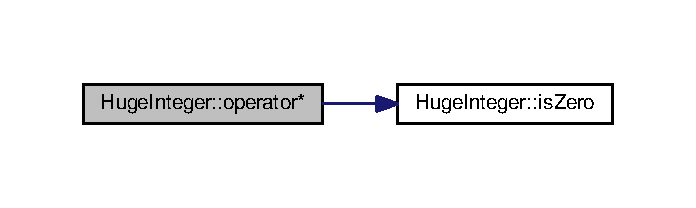
\includegraphics[width=334pt]{classHugeInteger_a40e338d499c8b70be27bf1e5dd0244c8_cgraph}
\end{center}
\end{figure}


\index{Huge\+Integer@{Huge\+Integer}!operator+@{operator+}}
\index{operator+@{operator+}!Huge\+Integer@{Huge\+Integer}}
\subsubsection[{\texorpdfstring{operator+(const Huge\+Integer \&h2) const }{operator+(const HugeInteger &h2) const }}]{\setlength{\rightskip}{0pt plus 5cm}{\bf Huge\+Integer} Huge\+Integer\+::operator+ (
\begin{DoxyParamCaption}
\item[{const {\bf Huge\+Integer} \&}]{h2}
\end{DoxyParamCaption}
) const}\hypertarget{classHugeInteger_a3b20d1fc01bc355958e11a286f988605}{}\label{classHugeInteger_a3b20d1fc01bc355958e11a286f988605}

\begin{DoxyCode}
136 \{
137    \hyperlink{classHugeInteger}{HugeInteger} ans;
138    vector<int> sum;
139    \textcolor{keywordtype}{int} length, number, carryOver = 0;
140    \textcolor{keywordflow}{if}(*\textcolor{keyword}{this} >= h2)
141       length = \hyperlink{classHugeInteger_a3d21e9f761dfb49fb6559389685af830}{num}.size();
142    \textcolor{keywordflow}{else}
143       length = h2.\hyperlink{classHugeInteger_a3d21e9f761dfb49fb6559389685af830}{num}.size();
144 
145    \textcolor{keywordflow}{for}(\textcolor{keywordtype}{int} k=0; k<length-1; k++)
146    \{
147       number = carryOver + \hyperlink{classHugeInteger_ab0bd42ce92321df91e3a9a11897cdb8a}{digits}[k] + h2.\hyperlink{classHugeInteger_ab0bd42ce92321df91e3a9a11897cdb8a}{digits}[k];
148       sum.push\_back(number%10); \textcolor{comment}{//the number on the ones place goes into sum                               
                                                                                                       }
149       carryOver = number/10; \textcolor{comment}{//the number in the tens place goes into carryOver}
150    \}
151 
152    number = carryOver + \hyperlink{classHugeInteger_ab0bd42ce92321df91e3a9a11897cdb8a}{digits}[length-1] + h2.\hyperlink{classHugeInteger_ab0bd42ce92321df91e3a9a11897cdb8a}{digits}[length-1];
153    sum.push\_back(number%10); \textcolor{comment}{//because the number is calculated backwards, the number in the ones place is
       added in first                                                                                   }
154    \textcolor{keywordflow}{if}(number/10 != 0)
155       sum.push\_back(number/10);
156 
157    \textcolor{keywordflow}{if}(\hyperlink{classHugeInteger_a714314b2e1b79827d8796d8c52016e5a}{overflow}(sum)) \textcolor{comment}{//if sum exceeds the limit size (MAXDIGITS), then a bad HugeInteger will be
       returned                                                                                                   }
158       ans = \hyperlink{classHugeInteger_a6d9c7e76adbd02057a8a4a1048e05870}{returnBad}();
159    \textcolor{keywordflow}{else}
160    \{
161       \hyperlink{classHugeInteger}{HugeInteger} hi(sum);
162       ans = hi;
163    \}
164 
165    \textcolor{keywordflow}{return} ans;
166 \}
\end{DoxyCode}
\index{Huge\+Integer@{Huge\+Integer}!operator-\/@{operator-\/}}
\index{operator-\/@{operator-\/}!Huge\+Integer@{Huge\+Integer}}
\subsubsection[{\texorpdfstring{operator-\/(const Huge\+Integer \&h2) const }{operator-(const HugeInteger &h2) const }}]{\setlength{\rightskip}{0pt plus 5cm}{\bf Huge\+Integer} Huge\+Integer\+::operator-\/ (
\begin{DoxyParamCaption}
\item[{const {\bf Huge\+Integer} \&}]{h2}
\end{DoxyParamCaption}
) const}\hypertarget{classHugeInteger_ad692378aa02c232eade02c4177984a20}{}\label{classHugeInteger_ad692378aa02c232eade02c4177984a20}

\begin{DoxyCode}
169 \{
170    vector<int> difference;
171    \textcolor{keywordtype}{int} a1[\hyperlink{classHugeInteger_a35ff958aa09161b192b69b1de876dab3}{MAXDIGITS}] = \{0\}, a2[\hyperlink{classHugeInteger_a35ff958aa09161b192b69b1de876dab3}{MAXDIGITS}] = \{0\};
172    \textcolor{keywordtype}{int} length, number, temp;
173    \textcolor{keywordtype}{char} s = \textcolor{charliteral}{'+'};
174    \hyperlink{classHugeInteger_a2b54adddc72d21bcd72126855db96188}{setUp}(h2, a1, a2, length, temp, s); \textcolor{comment}{//a1 and a2 are initialized depending on which HugeInteger is
       bigger                                                                                                 }
175 
176    \textcolor{keywordflow}{for}(\textcolor{keywordtype}{int} k=0; k<length; k++)
177    \{
178       \textcolor{keywordflow}{if}(a1[k] < a2[k])
179       \{
180          a1[k] += 10;
181          a1[k+1]--;
182       \}
183       difference.push\_back(a1[k] - a2[k]);
184    \}
185    \textcolor{keywordflow}{if}(difference.size() != 1)
186    \{
187       number = difference[difference.size()-1];
188       \textcolor{keywordflow}{while}(number == 0 && difference.size() != 1) \textcolor{comment}{//gets rid of excess zeros at the beginning of the
       vector (ex: 77 - 76 = 01)                                                                             }
189       \{
190          difference.pop\_back();
191          number = difference[difference.size()-1];
192       \}
193    \}
194 
195    \hyperlink{classHugeInteger}{HugeInteger} hi(difference, s);
196    \textcolor{keywordflow}{return} hi;
197 \}
\end{DoxyCode}
\index{Huge\+Integer@{Huge\+Integer}!operator$<$=@{operator$<$=}}
\index{operator$<$=@{operator$<$=}!Huge\+Integer@{Huge\+Integer}}
\subsubsection[{\texorpdfstring{operator$<$=(const Huge\+Integer \&h2) const }{operator<=(const HugeInteger &h2) const }}]{\setlength{\rightskip}{0pt plus 5cm}bool Huge\+Integer\+::operator$<$= (
\begin{DoxyParamCaption}
\item[{const {\bf Huge\+Integer} \&}]{h2}
\end{DoxyParamCaption}
) const}\hypertarget{classHugeInteger_a7cfb61d81ff41194b821ba51fe30a823}{}\label{classHugeInteger_a7cfb61d81ff41194b821ba51fe30a823}

\begin{DoxyCode}
290 \{
291    \textcolor{keywordflow}{return}(!(*\textcolor{keyword}{this} > h2)||(*\textcolor{keyword}{this} == h2));
292 \}
\end{DoxyCode}
\index{Huge\+Integer@{Huge\+Integer}!operator=@{operator=}}
\index{operator=@{operator=}!Huge\+Integer@{Huge\+Integer}}
\subsubsection[{\texorpdfstring{operator=(const Huge\+Integer \&h2)}{operator=(const HugeInteger &h2)}}]{\setlength{\rightskip}{0pt plus 5cm}{\bf Huge\+Integer} \& Huge\+Integer\+::operator= (
\begin{DoxyParamCaption}
\item[{const {\bf Huge\+Integer} \&}]{h2}
\end{DoxyParamCaption}
)}\hypertarget{classHugeInteger_a21b05accb9d8037d987361c569adcb34}{}\label{classHugeInteger_a21b05accb9d8037d987361c569adcb34}

\begin{DoxyCode}
58 \{
59    \textcolor{keywordflow}{for}(\textcolor{keywordtype}{int} k=0; k<\hyperlink{classHugeInteger_a35ff958aa09161b192b69b1de876dab3}{MAXDIGITS}; k++)
60       \hyperlink{classHugeInteger_ab0bd42ce92321df91e3a9a11897cdb8a}{digits}[k] = 0;
61    \textcolor{keywordflow}{for}(\textcolor{keywordtype}{int} k=0; k<\hyperlink{classHugeInteger_a35ff958aa09161b192b69b1de876dab3}{MAXDIGITS}; k++)
62       \hyperlink{classHugeInteger_ab0bd42ce92321df91e3a9a11897cdb8a}{digits}[k] = h2.\hyperlink{classHugeInteger_ab0bd42ce92321df91e3a9a11897cdb8a}{digits}[k];
63    \hyperlink{classHugeInteger_a3d21e9f761dfb49fb6559389685af830}{num}.erase(\hyperlink{classHugeInteger_a3d21e9f761dfb49fb6559389685af830}{num}.begin(), \hyperlink{classHugeInteger_a3d21e9f761dfb49fb6559389685af830}{num}.begin()+\hyperlink{classHugeInteger_a3d21e9f761dfb49fb6559389685af830}{num}.size());
64    \textcolor{keywordflow}{for}(\textcolor{keywordtype}{int} k=0; k<h2.\hyperlink{classHugeInteger_a3d21e9f761dfb49fb6559389685af830}{num}.size(); k++)
65       \hyperlink{classHugeInteger_a3d21e9f761dfb49fb6559389685af830}{num}.push\_back(h2.\hyperlink{classHugeInteger_a3d21e9f761dfb49fb6559389685af830}{num}[k]);
66    \hyperlink{classHugeInteger_a0ac2a85dbda0bd78e0df91fb6d6e2397}{sign} = h2.\hyperlink{classHugeInteger_a0ac2a85dbda0bd78e0df91fb6d6e2397}{sign};
67 
68    \textcolor{keywordflow}{return} *\textcolor{keyword}{this};
69 \}
\end{DoxyCode}
\index{Huge\+Integer@{Huge\+Integer}!operator==@{operator==}}
\index{operator==@{operator==}!Huge\+Integer@{Huge\+Integer}}
\subsubsection[{\texorpdfstring{operator==(const Huge\+Integer \&h2) const }{operator==(const HugeInteger &h2) const }}]{\setlength{\rightskip}{0pt plus 5cm}bool Huge\+Integer\+::operator== (
\begin{DoxyParamCaption}
\item[{const {\bf Huge\+Integer} \&}]{h2}
\end{DoxyParamCaption}
) const}\hypertarget{classHugeInteger_afd8c8c5e61cb6616dcd8672f187e3b98}{}\label{classHugeInteger_afd8c8c5e61cb6616dcd8672f187e3b98}

\begin{DoxyCode}
246 \{
247    \textcolor{keywordflow}{return} (!(*\textcolor{keyword}{this} > h2) && !(h2 > *\textcolor{keyword}{this}));
248 \}
\end{DoxyCode}
\index{Huge\+Integer@{Huge\+Integer}!operator$>$@{operator$>$}}
\index{operator$>$@{operator$>$}!Huge\+Integer@{Huge\+Integer}}
\subsubsection[{\texorpdfstring{operator$>$(const Huge\+Integer \&h2) const }{operator>(const HugeInteger &h2) const }}]{\setlength{\rightskip}{0pt plus 5cm}bool Huge\+Integer\+::operator$>$ (
\begin{DoxyParamCaption}
\item[{const {\bf Huge\+Integer} \&}]{h2}
\end{DoxyParamCaption}
) const\hspace{0.3cm}{\ttfamily [private]}}\hypertarget{classHugeInteger_a9ea6dc20120af0710d180f7fc2f15104}{}\label{classHugeInteger_a9ea6dc20120af0710d180f7fc2f15104}

\begin{DoxyCode}
256 \{
257    \textcolor{keywordtype}{int} count = 0;
258    \textcolor{keywordtype}{bool} greaterThan = \textcolor{keyword}{true};
259    \textcolor{keywordflow}{if}(\hyperlink{classHugeInteger_a3d21e9f761dfb49fb6559389685af830}{num}.size() < h2.\hyperlink{classHugeInteger_a3d21e9f761dfb49fb6559389685af830}{num}.size())
260       greaterThan = \textcolor{keyword}{false};
261    \textcolor{keywordflow}{else} \textcolor{keywordflow}{if}(\hyperlink{classHugeInteger_a3d21e9f761dfb49fb6559389685af830}{num}.size() == h2.\hyperlink{classHugeInteger_a3d21e9f761dfb49fb6559389685af830}{num}.size())
262    \{
263       \textcolor{keywordflow}{for}(\textcolor{keywordtype}{int} k=0; k<\hyperlink{classHugeInteger_a3d21e9f761dfb49fb6559389685af830}{num}.size(); k++)
264       \{
265          \textcolor{keywordflow}{if}(\hyperlink{classHugeInteger_a3d21e9f761dfb49fb6559389685af830}{num}[k] < h2.\hyperlink{classHugeInteger_a3d21e9f761dfb49fb6559389685af830}{num}[k])
266          \{
267             greaterThan = \textcolor{keyword}{false};
268             \textcolor{keywordflow}{break};
269          \}
270          \textcolor{keywordflow}{else} \textcolor{keywordflow}{if}(\hyperlink{classHugeInteger_a3d21e9f761dfb49fb6559389685af830}{num}[k] > h2.\hyperlink{classHugeInteger_a3d21e9f761dfb49fb6559389685af830}{num}[k])
271          \{
272             greaterThan = \textcolor{keyword}{true};
273             \textcolor{keywordflow}{break};
274          \}
275          \textcolor{keywordflow}{else}
276             count++;
277       \}
278       \textcolor{keywordflow}{if}(count == \hyperlink{classHugeInteger_a3d21e9f761dfb49fb6559389685af830}{num}.size())
279          greaterThan = \textcolor{keyword}{false};
280    \}
281    \textcolor{keywordflow}{return} greaterThan;
282 \}
\end{DoxyCode}
\index{Huge\+Integer@{Huge\+Integer}!operator$>$=@{operator$>$=}}
\index{operator$>$=@{operator$>$=}!Huge\+Integer@{Huge\+Integer}}
\subsubsection[{\texorpdfstring{operator$>$=(const Huge\+Integer \&h2) const }{operator>=(const HugeInteger &h2) const }}]{\setlength{\rightskip}{0pt plus 5cm}bool Huge\+Integer\+::operator$>$= (
\begin{DoxyParamCaption}
\item[{const {\bf Huge\+Integer} \&}]{h2}
\end{DoxyParamCaption}
) const}\hypertarget{classHugeInteger_a7e16c19293c8f8113cd4fb8a4d74d591}{}\label{classHugeInteger_a7e16c19293c8f8113cd4fb8a4d74d591}

\begin{DoxyCode}
285 \{
286    \textcolor{keywordflow}{return}((*\textcolor{keyword}{this} > h2)||(*\textcolor{keyword}{this} == h2));
287 \}
\end{DoxyCode}
\index{Huge\+Integer@{Huge\+Integer}!overflow@{overflow}}
\index{overflow@{overflow}!Huge\+Integer@{Huge\+Integer}}
\subsubsection[{\texorpdfstring{overflow(vector$<$ int $>$ v) const }{overflow(vector< int > v) const }}]{\setlength{\rightskip}{0pt plus 5cm}bool Huge\+Integer\+::overflow (
\begin{DoxyParamCaption}
\item[{vector$<$ int $>$}]{v}
\end{DoxyParamCaption}
) const\hspace{0.3cm}{\ttfamily [private]}}\hypertarget{classHugeInteger_a714314b2e1b79827d8796d8c52016e5a}{}\label{classHugeInteger_a714314b2e1b79827d8796d8c52016e5a}

\begin{DoxyCode}
100 \{
101    \textcolor{keywordflow}{return} (v.size() > \hyperlink{classHugeInteger_a35ff958aa09161b192b69b1de876dab3}{MAXDIGITS});
102 \}
\end{DoxyCode}
\index{Huge\+Integer@{Huge\+Integer}!overflow@{overflow}}
\index{overflow@{overflow}!Huge\+Integer@{Huge\+Integer}}
\subsubsection[{\texorpdfstring{overflow(vector$<$ char $>$ v) const }{overflow(vector< char > v) const }}]{\setlength{\rightskip}{0pt plus 5cm}bool Huge\+Integer\+::overflow (
\begin{DoxyParamCaption}
\item[{vector$<$ char $>$}]{v}
\end{DoxyParamCaption}
) const\hspace{0.3cm}{\ttfamily [private]}}\hypertarget{classHugeInteger_a5c25f70a6d5cdb5625de8b4990555ba0}{}\label{classHugeInteger_a5c25f70a6d5cdb5625de8b4990555ba0}

\begin{DoxyCode}
105 \{
106    \textcolor{keywordflow}{return} ((v.size() > \hyperlink{classHugeInteger_a35ff958aa09161b192b69b1de876dab3}{MAXDIGITS})||(v.size() == 0));
107 \}
\end{DoxyCode}
\index{Huge\+Integer@{Huge\+Integer}!return\+Bad@{return\+Bad}}
\index{return\+Bad@{return\+Bad}!Huge\+Integer@{Huge\+Integer}}
\subsubsection[{\texorpdfstring{return\+Bad() const }{returnBad() const }}]{\setlength{\rightskip}{0pt plus 5cm}{\bf Huge\+Integer} Huge\+Integer\+::return\+Bad (
\begin{DoxyParamCaption}
{}
\end{DoxyParamCaption}
) const\hspace{0.3cm}{\ttfamily [private]}}\hypertarget{classHugeInteger_a6d9c7e76adbd02057a8a4a1048e05870}{}\label{classHugeInteger_a6d9c7e76adbd02057a8a4a1048e05870}

\begin{DoxyCode}
91 \{
92    vector<int> f;
93    f.push\_back(0);
94    f.push\_back(0); \textcolor{comment}{//a bad HugeInteger has a vector of 00                                                  
                                                                                                       }
95    \hyperlink{classHugeInteger}{HugeInteger} fail(f);
96    \textcolor{keywordflow}{return} fail;
97 \}
\end{DoxyCode}
\index{Huge\+Integer@{Huge\+Integer}!set\+Up@{set\+Up}}
\index{set\+Up@{set\+Up}!Huge\+Integer@{Huge\+Integer}}
\subsubsection[{\texorpdfstring{set\+Up(const Huge\+Integer \&h, int a1[], int a2[], int \&len1, int \&len2, char \&s) const }{setUp(const HugeInteger &h, int a1[], int a2[], int &len1, int &len2, char &s) const }}]{\setlength{\rightskip}{0pt plus 5cm}void Huge\+Integer\+::set\+Up (
\begin{DoxyParamCaption}
\item[{const {\bf Huge\+Integer} \&}]{h, }
\item[{int}]{a1\mbox{[}$\,$\mbox{]}, }
\item[{int}]{a2\mbox{[}$\,$\mbox{]}, }
\item[{int \&}]{len1, }
\item[{int \&}]{len2, }
\item[{char \&}]{s}
\end{DoxyParamCaption}
) const\hspace{0.3cm}{\ttfamily [private]}}\hypertarget{classHugeInteger_a2b54adddc72d21bcd72126855db96188}{}\label{classHugeInteger_a2b54adddc72d21bcd72126855db96188}

\begin{DoxyCode}
111 \{
112    \textcolor{keywordflow}{if}(*\textcolor{keyword}{this} >= h)
113    \{
114       len1 = \hyperlink{classHugeInteger_a3d21e9f761dfb49fb6559389685af830}{num}.size();
115       len2 = h.\hyperlink{classHugeInteger_a3d21e9f761dfb49fb6559389685af830}{num}.size();
116       \textcolor{keywordflow}{for}(\textcolor{keywordtype}{int} m=0; m<\hyperlink{classHugeInteger_a35ff958aa09161b192b69b1de876dab3}{MAXDIGITS}; m++)
117       \{
118          a1[m] = \hyperlink{classHugeInteger_ab0bd42ce92321df91e3a9a11897cdb8a}{digits}[m]; \textcolor{comment}{//temporary arrays are given the same value as the digits array of the
       HugeIntegers so that they can be used interchangeably                                                    }
119          a2[m] = h.\hyperlink{classHugeInteger_ab0bd42ce92321df91e3a9a11897cdb8a}{digits}[m];
120       \}
121    \}
122    \textcolor{keywordflow}{else}
123    \{
124       len1 = h.\hyperlink{classHugeInteger_a3d21e9f761dfb49fb6559389685af830}{num}.size();
125       len2 = \hyperlink{classHugeInteger_a3d21e9f761dfb49fb6559389685af830}{num}.size();
126       \textcolor{keywordflow}{for}(\textcolor{keywordtype}{int} m=0; m<\hyperlink{classHugeInteger_a35ff958aa09161b192b69b1de876dab3}{MAXDIGITS}; m++)
127       \{
128          a1[m] = h.\hyperlink{classHugeInteger_ab0bd42ce92321df91e3a9a11897cdb8a}{digits}[m];
129          a2[m] = \hyperlink{classHugeInteger_ab0bd42ce92321df91e3a9a11897cdb8a}{digits}[m];
130       \}
131       s = \textcolor{charliteral}{'-'};
132    \}
133 \}
\end{DoxyCode}


\subsection{Friends And Related Function Documentation}
\index{Huge\+Integer@{Huge\+Integer}!Equation@{Equation}}
\index{Equation@{Equation}!Huge\+Integer@{Huge\+Integer}}
\subsubsection[{\texorpdfstring{Equation}{Equation}}]{\setlength{\rightskip}{0pt plus 5cm}friend class Equation\hspace{0.3cm}{\ttfamily [friend]}}\hypertarget{classHugeInteger_a9bfba8577640e06376146eaf7da56aae}{}\label{classHugeInteger_a9bfba8577640e06376146eaf7da56aae}
\index{Huge\+Integer@{Huge\+Integer}!operator$<$$<$@{operator$<$$<$}}
\index{operator$<$$<$@{operator$<$$<$}!Huge\+Integer@{Huge\+Integer}}
\subsubsection[{\texorpdfstring{operator$<$$<$}{operator<<}}]{\setlength{\rightskip}{0pt plus 5cm}ostream\& operator$<$$<$ (
\begin{DoxyParamCaption}
\item[{ostream \&}]{outs, }
\item[{const {\bf Huge\+Integer} \&}]{hi}
\end{DoxyParamCaption}
)\hspace{0.3cm}{\ttfamily [friend]}}\hypertarget{classHugeInteger_aa9a08688da0c2e4f6983a36161b3d008}{}\label{classHugeInteger_aa9a08688da0c2e4f6983a36161b3d008}

\begin{DoxyCode}
295 \{
296    \textcolor{keywordflow}{if}(hi.\hyperlink{classHugeInteger_a0ac2a85dbda0bd78e0df91fb6d6e2397}{sign} == \textcolor{charliteral}{'-'})
297       cout << hi.\hyperlink{classHugeInteger_a0ac2a85dbda0bd78e0df91fb6d6e2397}{sign};
298    \textcolor{keywordflow}{for}(\textcolor{keywordtype}{int} k=0; k<hi.\hyperlink{classHugeInteger_a3d21e9f761dfb49fb6559389685af830}{num}.size(); k++)
299       outs << hi.\hyperlink{classHugeInteger_a3d21e9f761dfb49fb6559389685af830}{num}[k];
300    \textcolor{keywordflow}{return} outs;
301 \}
\end{DoxyCode}
\index{Huge\+Integer@{Huge\+Integer}!operator$>$$>$@{operator$>$$>$}}
\index{operator$>$$>$@{operator$>$$>$}!Huge\+Integer@{Huge\+Integer}}
\subsubsection[{\texorpdfstring{operator$>$$>$}{operator>>}}]{\setlength{\rightskip}{0pt plus 5cm}istream\& operator$>$$>$ (
\begin{DoxyParamCaption}
\item[{istream \&}]{ins, }
\item[{{\bf Huge\+Integer} \&}]{hi}
\end{DoxyParamCaption}
)\hspace{0.3cm}{\ttfamily [friend]}}\hypertarget{classHugeInteger_afeff4742c40990020c005d43e8de8e64}{}\label{classHugeInteger_afeff4742c40990020c005d43e8de8e64}

\begin{DoxyCode}
304 \{
305    \textcolor{keywordtype}{char} c, d;
306    \textcolor{keywordtype}{int} i;
307    vector<char> v;
308 
309    \textcolor{keywordflow}{do} \textcolor{comment}{//weeds through input until a number or comma is found                                               
                                                                                                       }
310    \{
311       ins >> c;
312       i = c;\textcolor{comment}{// converts c into an integer using the ASCII value chart                                      
                                                                                                       }
313    \}\textcolor{keywordflow}{while}(!((i >= 48 && i <= 57)||(i == 44)));
314 
315    ins.putback(c); \textcolor{comment}{//puts retrieved input value back so that another variable can retrieve it              
                                                                                                       }
316 
317    \textcolor{keywordflow}{while}((i >= 48 && i <= 57)||(i == 44)) \textcolor{comment}{//48 - 57 corresponds to characters 0-9 and 44 corresponds to the
       comma character                                                                                 }
318    \{
319       ins >> d;
320       \textcolor{keywordflow}{if}(i >= 48 && i <=57) \textcolor{comment}{//excludes commas from the vector                                              
                                                                                                       }
321          v.push\_back(d);
322       c = ins.peek(); \textcolor{comment}{//sees the first input value, but does not retrieve it                               
                                                                                                       }
323       i = c;
324    \}
325 
326    \textcolor{keywordflow}{if}(hi.\hyperlink{classHugeInteger_a714314b2e1b79827d8796d8c52016e5a}{overflow}(v)) \textcolor{comment}{//if the input vector's size exceeds MAXDIGITS, a bad HugeInteger will be
       returned                                                                                                    }
327       hi = hi.\hyperlink{classHugeInteger_a6d9c7e76adbd02057a8a4a1048e05870}{returnBad}();
328    \textcolor{keywordflow}{else}
329    \{
330       \hyperlink{classHugeInteger}{HugeInteger} h(v);
331       hi = h;
332    \}
333 
334    \textcolor{keywordflow}{return} ins;
335 \}
\end{DoxyCode}


\subsection{Member Data Documentation}
\index{Huge\+Integer@{Huge\+Integer}!digits@{digits}}
\index{digits@{digits}!Huge\+Integer@{Huge\+Integer}}
\subsubsection[{\texorpdfstring{digits}{digits}}]{\setlength{\rightskip}{0pt plus 5cm}int Huge\+Integer\+::digits\mbox{[}{\bf M\+A\+X\+D\+I\+G\+I\+TS}\mbox{]}\hspace{0.3cm}{\ttfamily [private]}}\hypertarget{classHugeInteger_ab0bd42ce92321df91e3a9a11897cdb8a}{}\label{classHugeInteger_ab0bd42ce92321df91e3a9a11897cdb8a}
\index{Huge\+Integer@{Huge\+Integer}!M\+A\+X\+D\+I\+G\+I\+TS@{M\+A\+X\+D\+I\+G\+I\+TS}}
\index{M\+A\+X\+D\+I\+G\+I\+TS@{M\+A\+X\+D\+I\+G\+I\+TS}!Huge\+Integer@{Huge\+Integer}}
\subsubsection[{\texorpdfstring{M\+A\+X\+D\+I\+G\+I\+TS}{MAXDIGITS}}]{\setlength{\rightskip}{0pt plus 5cm}const int Huge\+Integer\+::\+M\+A\+X\+D\+I\+G\+I\+TS = 40\hspace{0.3cm}{\ttfamily [static]}, {\ttfamily [private]}}\hypertarget{classHugeInteger_a35ff958aa09161b192b69b1de876dab3}{}\label{classHugeInteger_a35ff958aa09161b192b69b1de876dab3}
\index{Huge\+Integer@{Huge\+Integer}!num@{num}}
\index{num@{num}!Huge\+Integer@{Huge\+Integer}}
\subsubsection[{\texorpdfstring{num}{num}}]{\setlength{\rightskip}{0pt plus 5cm}vector$<$int$>$ Huge\+Integer\+::num\hspace{0.3cm}{\ttfamily [private]}}\hypertarget{classHugeInteger_a3d21e9f761dfb49fb6559389685af830}{}\label{classHugeInteger_a3d21e9f761dfb49fb6559389685af830}
\index{Huge\+Integer@{Huge\+Integer}!sign@{sign}}
\index{sign@{sign}!Huge\+Integer@{Huge\+Integer}}
\subsubsection[{\texorpdfstring{sign}{sign}}]{\setlength{\rightskip}{0pt plus 5cm}char Huge\+Integer\+::sign\hspace{0.3cm}{\ttfamily [private]}}\hypertarget{classHugeInteger_a0ac2a85dbda0bd78e0df91fb6d6e2397}{}\label{classHugeInteger_a0ac2a85dbda0bd78e0df91fb6d6e2397}


The documentation for this class was generated from the following files\+:\begin{DoxyCompactItemize}
\item 
\hyperlink{HugeInteger_8h}{Huge\+Integer.\+h}\item 
\hyperlink{HugeInteger_8cpp}{Huge\+Integer.\+cpp}\end{DoxyCompactItemize}

\chapter{File Documentation}
\hypertarget{Emain_8cpp}{}\section{Emain.\+cpp File Reference}
\label{Emain_8cpp}\index{Emain.\+cpp@{Emain.\+cpp}}
{\ttfamily \#include $<$iostream$>$}\\*
{\ttfamily \#include \char`\"{}Equation.\+h\char`\"{}}\\*
{\ttfamily \#include \char`\"{}Huge\+Integer.\+h\char`\"{}}\\*
Include dependency graph for Emain.\+cpp\+:
\nopagebreak
\begin{figure}[H]
\begin{center}
\leavevmode
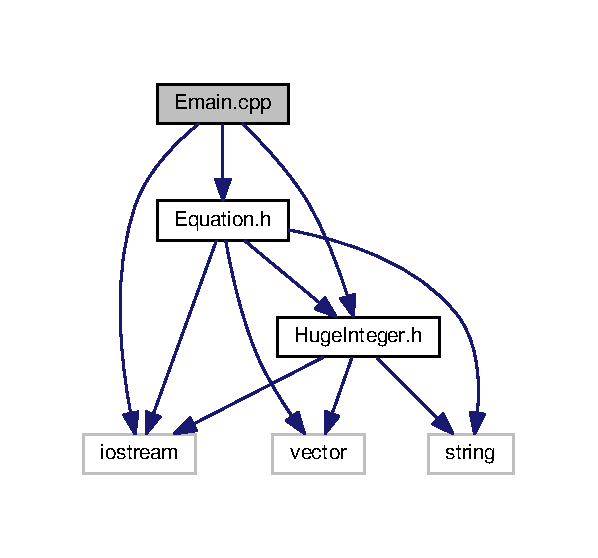
\includegraphics[width=287pt]{Emain_8cpp__incl}
\end{center}
\end{figure}
\subsection*{Functions}
\begin{DoxyCompactItemize}
\item 
int \hyperlink{Emain_8cpp_ae66f6b31b5ad750f1fe042a706a4e3d4}{main} ()
\end{DoxyCompactItemize}


\subsection{Function Documentation}
\index{Emain.\+cpp@{Emain.\+cpp}!main@{main}}
\index{main@{main}!Emain.\+cpp@{Emain.\+cpp}}
\subsubsection[{\texorpdfstring{main()}{main()}}]{\setlength{\rightskip}{0pt plus 5cm}int main (
\begin{DoxyParamCaption}
{}
\end{DoxyParamCaption}
)}\hypertarget{Emain_8cpp_ae66f6b31b5ad750f1fe042a706a4e3d4}{}\label{Emain_8cpp_ae66f6b31b5ad750f1fe042a706a4e3d4}

\begin{DoxyCode}
12 \{
13    \hyperlink{classEquation}{Equation} e;
14 
15    cout << endl << \textcolor{stringliteral}{"Enter an equation: "};
16    cin >> e;
17 
18    \textcolor{keywordflow}{while}(!e.end()) \textcolor{comment}{//if user enters 0x0, e.end will be true                                                
                                                                                                       }
19    \{
20       e.\hyperlink{classEquation_ab5694559600529bd6da9bb37428bfc5d}{calculate}(); \textcolor{comment}{//calculates the equation requested by the user and displays the result      
                                                                                                                }
21       cout << \textcolor{stringliteral}{"Enter another equation (or 0x0 to exit): "};
22       cin >> e;
23    \}
24 
25    \textcolor{keywordflow}{return} 0;
26 \}
\end{DoxyCode}


Here is the call graph for this function\+:
\nopagebreak
\begin{figure}[H]
\begin{center}
\leavevmode
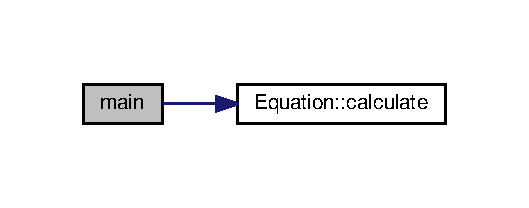
\includegraphics[width=254pt]{Emain_8cpp_ae66f6b31b5ad750f1fe042a706a4e3d4_cgraph}
\end{center}
\end{figure}



\hypertarget{Equation_8cpp}{}\section{Equation.\+cpp File Reference}
\label{Equation_8cpp}\index{Equation.\+cpp@{Equation.\+cpp}}
{\ttfamily \#include $<$iostream$>$}\\*
{\ttfamily \#include \char`\"{}Equation.\+h\char`\"{}}\\*
{\ttfamily \#include \char`\"{}Huge\+Integer.\+h\char`\"{}}\\*
Include dependency graph for Equation.\+cpp\+:
\nopagebreak
\begin{figure}[H]
\begin{center}
\leavevmode
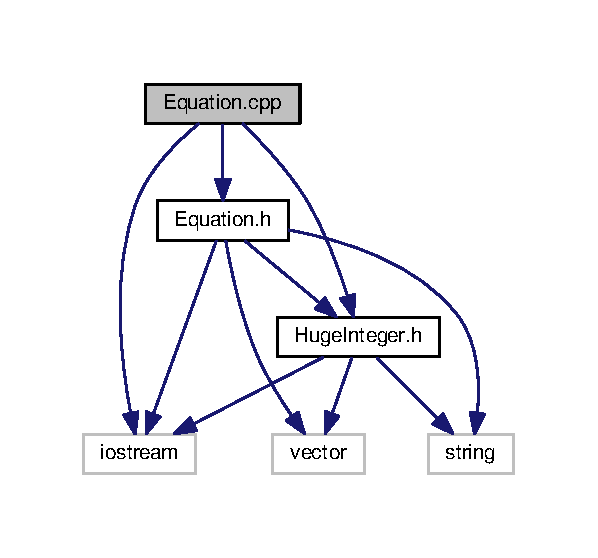
\includegraphics[width=287pt]{Equation_8cpp__incl}
\end{center}
\end{figure}
\subsection*{Functions}
\begin{DoxyCompactItemize}
\item 
ostream \& \hyperlink{Equation_8cpp_a6d50068fecbcab1522c61543256b4ae8}{operator$<$$<$} (ostream \&outs, const \hyperlink{classEquation}{Equation} \&e)
\item 
istream \& \hyperlink{Equation_8cpp_a6ba26a194f6be34f5f14611146f49312}{operator$>$$>$} (istream \&ins, \hyperlink{classEquation}{Equation} \&e)
\end{DoxyCompactItemize}


\subsection{Function Documentation}
\index{Equation.\+cpp@{Equation.\+cpp}!operator$<$$<$@{operator$<$$<$}}
\index{operator$<$$<$@{operator$<$$<$}!Equation.\+cpp@{Equation.\+cpp}}
\subsubsection[{\texorpdfstring{operator$<$$<$(ostream \&outs, const Equation \&e)}{operator<<(ostream &outs, const Equation &e)}}]{\setlength{\rightskip}{0pt plus 5cm}ostream\& operator$<$$<$ (
\begin{DoxyParamCaption}
\item[{ostream \&}]{outs, }
\item[{const {\bf Equation} \&}]{e}
\end{DoxyParamCaption}
)}\hypertarget{Equation_8cpp_a6d50068fecbcab1522c61543256b4ae8}{}\label{Equation_8cpp_a6d50068fecbcab1522c61543256b4ae8}

\begin{DoxyCode}
98 \{
99    \textcolor{keywordflow}{if}(e.\hyperlink{classEquation_a4d9ef234f54586c639efa69d7e958760}{sign} == \textcolor{charliteral}{'+'} || e.\hyperlink{classEquation_a4d9ef234f54586c639efa69d7e958760}{sign} == \textcolor{charliteral}{'*'} || e.\hyperlink{classEquation_a4d9ef234f54586c639efa69d7e958760}{sign} == \textcolor{charliteral}{'-'}) \textcolor{comment}{//if the operation was +,*, or -, the
       anser will have a result                                                                                      
       }
100       outs << endl << e.\hyperlink{classEquation_af03ee24dda87646ad14a87363fe6a459}{op1} << \textcolor{stringliteral}{" "} << e.\hyperlink{classEquation_a4d9ef234f54586c639efa69d7e958760}{sign} << \textcolor{stringliteral}{" "} << e.\hyperlink{classEquation_ab437f2357b6156b3e70c195cbb9304a5}{op2} << \textcolor{stringliteral}{" = "} << e.
      \hyperlink{classEquation_a7696f7ad262ed21259b3fd3d2d628549}{result} << endl << endl;
101    \textcolor{keywordflow}{else} \textcolor{comment}{//for the comparison operators                                                                     
                                                                                                       }
102       outs << endl << e.\hyperlink{classEquation_af03ee24dda87646ad14a87363fe6a459}{op1} << \textcolor{stringliteral}{" "} << e.\hyperlink{classEquation_a4d9ef234f54586c639efa69d7e958760}{sign} << \textcolor{stringliteral}{"= "} << e.\hyperlink{classEquation_ab437f2357b6156b3e70c195cbb9304a5}{op2} << \textcolor{stringliteral}{" "};
103    \textcolor{keywordflow}{return} outs;
104 \}
\end{DoxyCode}
\index{Equation.\+cpp@{Equation.\+cpp}!operator$>$$>$@{operator$>$$>$}}
\index{operator$>$$>$@{operator$>$$>$}!Equation.\+cpp@{Equation.\+cpp}}
\subsubsection[{\texorpdfstring{operator$>$$>$(istream \&ins, Equation \&e)}{operator>>(istream &ins, Equation &e)}}]{\setlength{\rightskip}{0pt plus 5cm}istream\& operator$>$$>$ (
\begin{DoxyParamCaption}
\item[{istream \&}]{ins, }
\item[{{\bf Equation} \&}]{e}
\end{DoxyParamCaption}
)}\hypertarget{Equation_8cpp_a6ba26a194f6be34f5f14611146f49312}{}\label{Equation_8cpp_a6ba26a194f6be34f5f14611146f49312}

\begin{DoxyCode}
107 \{
108    \textcolor{keywordtype}{bool} c;
109    \textcolor{keywordtype}{char} s;
110    \hyperlink{classHugeInteger}{HugeInteger} h1, h2;
111 
112    ins >> h1 >> s >> h2;
113    \textcolor{keywordflow}{if}(h1.\hyperlink{classHugeInteger_a49c11f16dad4dbb56d277ddb0eb71342}{isBad}() || h2.isBad()) \textcolor{comment}{//registers that the equation is bad                                  
                                                                                                            }
114       c = \textcolor{keyword}{false};
115    \textcolor{keywordflow}{else}
116       c = \textcolor{keyword}{true};
117 
118    \hyperlink{classEquation}{Equation} temp(h1, h2, s, c);
119    e = temp;
120 
121    \textcolor{keywordflow}{return} ins;
122 \}
\end{DoxyCode}


Here is the call graph for this function\+:
\nopagebreak
\begin{figure}[H]
\begin{center}
\leavevmode
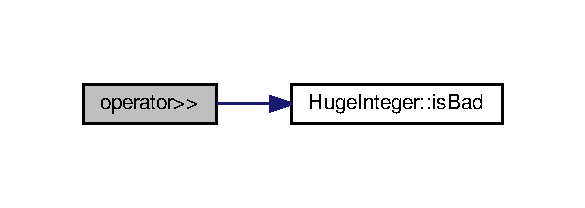
\includegraphics[width=281pt]{Equation_8cpp_a6ba26a194f6be34f5f14611146f49312_cgraph}
\end{center}
\end{figure}



\hypertarget{Equation_8h}{}\section{Equation.\+h File Reference}
\label{Equation_8h}\index{Equation.\+h@{Equation.\+h}}
{\ttfamily \#include $<$iostream$>$}\\*
{\ttfamily \#include $<$string$>$}\\*
{\ttfamily \#include $<$vector$>$}\\*
{\ttfamily \#include \char`\"{}Huge\+Integer.\+h\char`\"{}}\\*
Include dependency graph for Equation.\+h\+:
\nopagebreak
\begin{figure}[H]
\begin{center}
\leavevmode
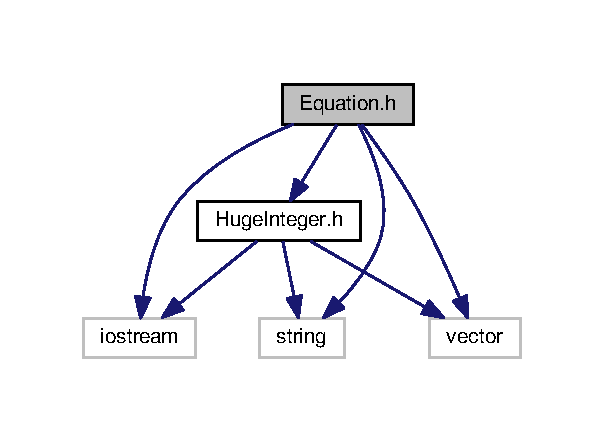
\includegraphics[width=290pt]{Equation_8h__incl}
\end{center}
\end{figure}
This graph shows which files directly or indirectly include this file\+:
\nopagebreak
\begin{figure}[H]
\begin{center}
\leavevmode
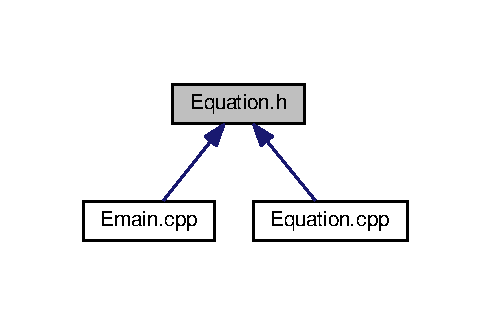
\includegraphics[width=236pt]{Equation_8h__dep__incl}
\end{center}
\end{figure}
\subsection*{Classes}
\begin{DoxyCompactItemize}
\item 
class \hyperlink{classEquation}{Equation}
\end{DoxyCompactItemize}

\hypertarget{HugeInteger_8cpp}{}\section{Huge\+Integer.\+cpp File Reference}
\label{HugeInteger_8cpp}\index{Huge\+Integer.\+cpp@{Huge\+Integer.\+cpp}}
{\ttfamily \#include $<$iostream$>$}\\*
{\ttfamily \#include $<$string$>$}\\*
{\ttfamily \#include $<$vector$>$}\\*
{\ttfamily \#include \char`\"{}Huge\+Integer.\+h\char`\"{}}\\*
Include dependency graph for Huge\+Integer.\+cpp\+:
\nopagebreak
\begin{figure}[H]
\begin{center}
\leavevmode
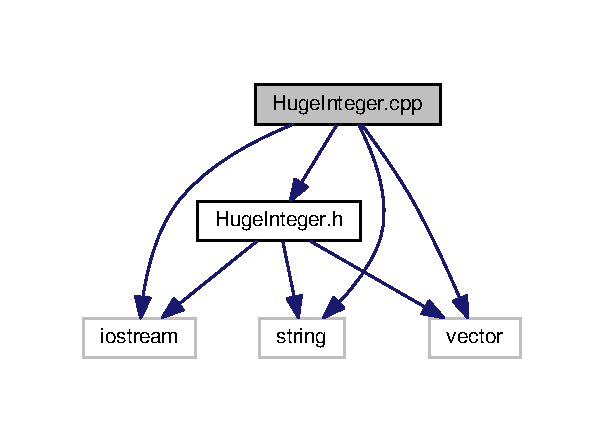
\includegraphics[width=290pt]{HugeInteger_8cpp__incl}
\end{center}
\end{figure}
\subsection*{Functions}
\begin{DoxyCompactItemize}
\item 
ostream \& \hyperlink{HugeInteger_8cpp_aa9a08688da0c2e4f6983a36161b3d008}{operator$<$$<$} (ostream \&outs, const \hyperlink{classHugeInteger}{Huge\+Integer} \&hi)
\item 
istream \& \hyperlink{HugeInteger_8cpp_afeff4742c40990020c005d43e8de8e64}{operator$>$$>$} (istream \&ins, \hyperlink{classHugeInteger}{Huge\+Integer} \&hi)
\end{DoxyCompactItemize}


\subsection{Function Documentation}
\index{Huge\+Integer.\+cpp@{Huge\+Integer.\+cpp}!operator$<$$<$@{operator$<$$<$}}
\index{operator$<$$<$@{operator$<$$<$}!Huge\+Integer.\+cpp@{Huge\+Integer.\+cpp}}
\subsubsection[{\texorpdfstring{operator$<$$<$(ostream \&outs, const Huge\+Integer \&hi)}{operator<<(ostream &outs, const HugeInteger &hi)}}]{\setlength{\rightskip}{0pt plus 5cm}ostream\& operator$<$$<$ (
\begin{DoxyParamCaption}
\item[{ostream \&}]{outs, }
\item[{const {\bf Huge\+Integer} \&}]{hi}
\end{DoxyParamCaption}
)}\hypertarget{HugeInteger_8cpp_aa9a08688da0c2e4f6983a36161b3d008}{}\label{HugeInteger_8cpp_aa9a08688da0c2e4f6983a36161b3d008}

\begin{DoxyCode}
295 \{
296    \textcolor{keywordflow}{if}(hi.\hyperlink{classHugeInteger_a0ac2a85dbda0bd78e0df91fb6d6e2397}{sign} == \textcolor{charliteral}{'-'})
297       cout << hi.\hyperlink{classHugeInteger_a0ac2a85dbda0bd78e0df91fb6d6e2397}{sign};
298    \textcolor{keywordflow}{for}(\textcolor{keywordtype}{int} k=0; k<hi.\hyperlink{classHugeInteger_a3d21e9f761dfb49fb6559389685af830}{num}.size(); k++)
299       outs << hi.\hyperlink{classHugeInteger_a3d21e9f761dfb49fb6559389685af830}{num}[k];
300    \textcolor{keywordflow}{return} outs;
301 \}
\end{DoxyCode}
\index{Huge\+Integer.\+cpp@{Huge\+Integer.\+cpp}!operator$>$$>$@{operator$>$$>$}}
\index{operator$>$$>$@{operator$>$$>$}!Huge\+Integer.\+cpp@{Huge\+Integer.\+cpp}}
\subsubsection[{\texorpdfstring{operator$>$$>$(istream \&ins, Huge\+Integer \&hi)}{operator>>(istream &ins, HugeInteger &hi)}}]{\setlength{\rightskip}{0pt plus 5cm}istream\& operator$>$$>$ (
\begin{DoxyParamCaption}
\item[{istream \&}]{ins, }
\item[{{\bf Huge\+Integer} \&}]{hi}
\end{DoxyParamCaption}
)}\hypertarget{HugeInteger_8cpp_afeff4742c40990020c005d43e8de8e64}{}\label{HugeInteger_8cpp_afeff4742c40990020c005d43e8de8e64}

\begin{DoxyCode}
304 \{
305    \textcolor{keywordtype}{char} c, d;
306    \textcolor{keywordtype}{int} i;
307    vector<char> v;
308 
309    \textcolor{keywordflow}{do} \textcolor{comment}{//weeds through input until a number or comma is found                                               
                                                                                                       }
310    \{
311       ins >> c;
312       i = c;\textcolor{comment}{// converts c into an integer using the ASCII value chart                                      
                                                                                                       }
313    \}\textcolor{keywordflow}{while}(!((i >= 48 && i <= 57)||(i == 44)));
314 
315    ins.putback(c); \textcolor{comment}{//puts retrieved input value back so that another variable can retrieve it              
                                                                                                       }
316 
317    \textcolor{keywordflow}{while}((i >= 48 && i <= 57)||(i == 44)) \textcolor{comment}{//48 - 57 corresponds to characters 0-9 and 44 corresponds to the
       comma character                                                                                 }
318    \{
319       ins >> d;
320       \textcolor{keywordflow}{if}(i >= 48 && i <=57) \textcolor{comment}{//excludes commas from the vector                                              
                                                                                                       }
321          v.push\_back(d);
322       c = ins.peek(); \textcolor{comment}{//sees the first input value, but does not retrieve it                               
                                                                                                       }
323       i = c;
324    \}
325 
326    \textcolor{keywordflow}{if}(hi.\hyperlink{classHugeInteger_a714314b2e1b79827d8796d8c52016e5a}{overflow}(v)) \textcolor{comment}{//if the input vector's size exceeds MAXDIGITS, a bad HugeInteger will be
       returned                                                                                                    }
327       hi = hi.\hyperlink{classHugeInteger_a6d9c7e76adbd02057a8a4a1048e05870}{returnBad}();
328    \textcolor{keywordflow}{else}
329    \{
330       \hyperlink{classHugeInteger}{HugeInteger} h(v);
331       hi = h;
332    \}
333 
334    \textcolor{keywordflow}{return} ins;
335 \}
\end{DoxyCode}


Here is the call graph for this function\+:
\nopagebreak
\begin{figure}[H]
\begin{center}
\leavevmode
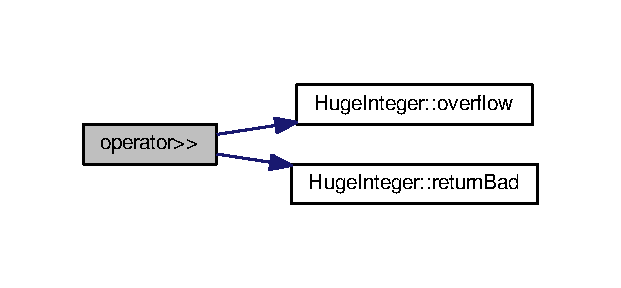
\includegraphics[width=298pt]{HugeInteger_8cpp_afeff4742c40990020c005d43e8de8e64_cgraph}
\end{center}
\end{figure}



\hypertarget{HugeInteger_8h}{}\section{Huge\+Integer.\+h File Reference}
\label{HugeInteger_8h}\index{Huge\+Integer.\+h@{Huge\+Integer.\+h}}
{\ttfamily \#include $<$iostream$>$}\\*
{\ttfamily \#include $<$string$>$}\\*
{\ttfamily \#include $<$vector$>$}\\*
Include dependency graph for Huge\+Integer.\+h\+:
\nopagebreak
\begin{figure}[H]
\begin{center}
\leavevmode
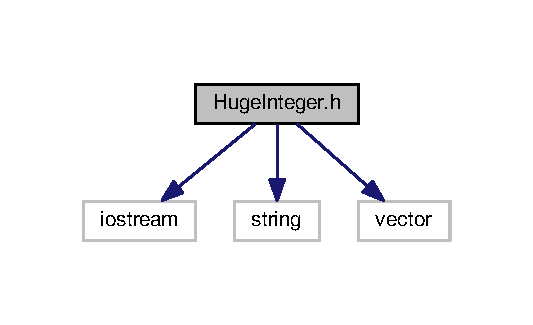
\includegraphics[width=256pt]{HugeInteger_8h__incl}
\end{center}
\end{figure}
This graph shows which files directly or indirectly include this file\+:
\nopagebreak
\begin{figure}[H]
\begin{center}
\leavevmode
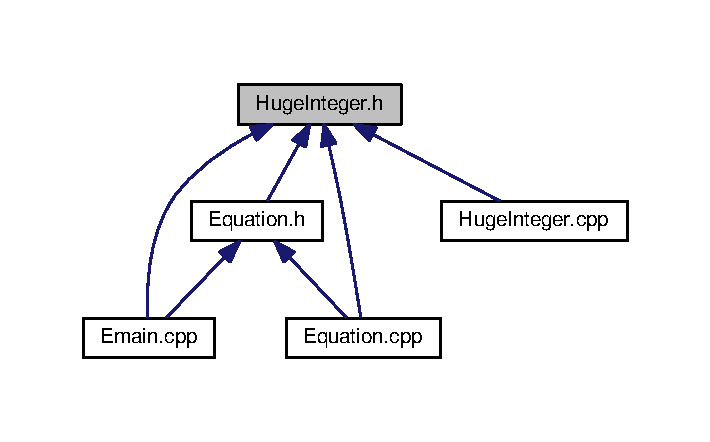
\includegraphics[width=341pt]{HugeInteger_8h__dep__incl}
\end{center}
\end{figure}
\subsection*{Classes}
\begin{DoxyCompactItemize}
\item 
class \hyperlink{classHugeInteger}{Huge\+Integer}
\end{DoxyCompactItemize}

%--- End generated contents ---

% Index
\backmatter
\newpage
\phantomsection
\clearemptydoublepage
\addcontentsline{toc}{chapter}{Index}
\printindex

\end{document}
